\documentclass[a4paper,10pt,oneside]{article}
\usepackage[polutonikogreek,italian]{babel}
\usepackage[utf8x]{inputenc}
\usepackage{amsmath}
\usepackage{amsthm}
\usepackage{amssymb}
\usepackage{amscd}
\usepackage{graphicx}
\usepackage{float}
\usepackage{array}
\usepackage{rotating}
\usepackage[small]{caption}
\usepackage{lscape}
\usepackage{fancybox}
\usepackage{booktabs}
\parindent0ex 
\renewcommand{\fboxsep}{0.5cm}
\usepackage{hyperref}
\renewcommand{\textfraction}{0.05}
\renewcommand{\topfraction}{0.95}
\renewcommand{\bottomfraction}{0.95}
\renewcommand{\floatpagefraction}{0.35}
\setcounter{totalnumber}{5}
\restylefloat{figure}
\newlength{\drop}
\begin{document}

\begin{center}
{\huge Laboratorio di cinematica bidimensionale}
\end{center}

\begin{abstract}
In questo laboratorio studieremo il moto parabolico ed il moto circolare  tramite l'osservazione della traiettoria di un corpo (quasi) puntiforme.
\end{abstract}


\vspace{1.5cm}


\section{Moto parabolico}

Per studiare il moto di un proiettile utilizzeremo un cannone ad elastico come in figura [\ref{fig:cannone1}]
\begin{figure}[H]
 \centering
 \includegraphics[width=\textwidth]{./Immagini/cannone.png}
 % cannone.png: 1808x1119 pixel, 500dpi, 9.19x5.69 cm, bb=
 \caption{Cannone ad elastico montato in laboratorio}
 \label{fig:cannone1}
\end{figure}
Durante gli esperimenti la bocca del cannone si troverà ad una quota $y$, l'inclinazione del tubo di lancio sarà $\theta$ e la velocità iniziale del proiettile sarà $v_0$. Le componenti della velocità $\mathbf{v}(t)$ saranno:
\begin{align}
 v_x(t)&=v_0\cos \theta\\
 v_y(t)&=v_0\sin\theta -gt
\end{align}
dove $g$ è l'accelerazione di gravità. Le componenti dello spostamento saranno:
\begin{align}\label{posizione}
 x(t)&=v_0t\cos\theta\\
 y(t)&=y_0+v_0t\sin \theta -\frac{1}{2} g t^2
\end{align}

dove si è presupposto che la bocca del cannone si trovi alle coordinate $x=0$ e $y=y_0$. Dalle [\ref{posizione}] possiamo ricavare facilmente la distanza $L$ dalla bocca del cannone ad un istante $t$:
\begin{equation}
 L(t)=\sqrt{(v_0 t\cos\theta )^2+(y_0+v_0t \sin \theta-\frac 1 2 g t^2)^2}
\end{equation}

e la gittata in  funzione dell'angolo $\theta$:
\begin{equation}
 g(\theta)=v_0\cos \theta\frac{v_0\sin\theta+\sqrt{v^2\sin^2\theta+2 y_0 g}}{g}
\end{equation}
avremo gittata massima per un angolo $\theta$:
\begin{equation}
 \theta_{max}=\arccos\sqrt{\frac{v_0^2+2gy_0}{2v_0^2+2gy_0}}
\end{equation}

possiamo notare che se $y_0=0$ allora $\theta_{max}=\arccos\frac{1}{\sqrt 2}=\pi/4$ 
\begin{figure}[H]
 \centering
 \includegraphics[width=\textwidth]{./Immagini/gittata1.pdf}
 % gittata1.pdf: 673x428 pixel, 72dpi, 23.74x15.10 cm, bb=
 \caption{Gittata in funzione dell'angolo $\theta$ e della posizione iniziale $y_0$ del proiettile. Velocità iniziale $v_0=2ms^{-1}$ e $0<y_0<0.5 m$}
 \label{fig:gittata_variazione}
\end{figure}

Tutti calcoli presentati precedentemente si suppongono svolti in assenza di atmosfera, considerando la terra un sistema inerziale e l'accelerazione di gravità costante; per tali motivi i risultati sperimentali si discosteranno dalle previsioni teoriche presentate precedentemente.
\subsection{Determinazione della traiettoria}
Per determinare la traiettoria del proiettile lanciato dal cannone ad elastico,  utilizzeremo una macchina fotografica digitale in grado di riprendere filmati ad alta velocità. 
\begin{figure}[H]
 \centering
 \includegraphics[width=\textwidth]{./Immagini/cannone3.png}
 % cannone3.png: 4339x1123 pixel, 500dpi, 22.05x5.71 cm, bb=
 \caption{La traiettoria sarà determinata misurando le successive posizioni del centro della pallina.}
 \label{fig:cannone3}
\end{figure}
Procederemo nel modo seguente:
\begin{itemize}
 \item Impostiamo la frequenza di campionamento della macchina fotografica (es 120Hz)
\item Riprendiamo il moto per una data estrazione del pistone del cannone.
\item Ripetiamo la ripresa per tre volte (ad allungamento fisso dell'elastico)
\end{itemize}
I filmati ripresi dovranno essere poi elaborati seguendo la guida che sarà pubblicata dopo il laboratorio all'indirizzo \url{http://cartan.e-moka.net}.

\subsection{Determinazione della gittata}

Per determinare di quanto la previsione teorica si discosta dalla realtà dobbiamo misurare la velocità iniziale del proiettile, l'inclinazione del cannone ed il punto di impatto del proiettile con il banco del laboratorio. 
Il sensore di moto della pasco verrà posizionato orizzontalmente e misurerà la variazione della posizione $x$ del proiettile negli istanti immediatamente successivi al lancio. Conoscendo l'inclinazione del cannone saremo quindi in grado di calcolare il modulo della velocità iniziale della pallina.
\begin{figure}[H]
 \centering
 \includegraphics[width=\textwidth]{./Immagini/cannone5.png}
 % cannone5.png: 4339x1333 pixel, 500dpi, 22.05x6.77 cm, bb=
 \caption{Posizionamento del sensore di moto Pasco per la misurazione della velocità iniziale del proiettile}
 \label{fig:cannone4}
\end{figure}

\section{Moto circolare}

Un moto circolare uniforme può essere espresso tramite la velocità angolare $\omega=2\pi \nu$ e la distanza $r$ dal centro. Siccome studieremo unicamente moti uniformi sarà:
\begin{equation}
 \frac{d\omega}{dt}=0
\end{equation}
il vettore posizione potrà essere espresso come:
\begin{align}
 x(t)&=r\cos(\omega t)\\
y(t)&=r\sin(\omega t)
\end{align}
mentre le componenti della velocità saranno:
\begin{align}
 v_x(t)&=-r\omega\sin(\omega t)\\
v_y(t)&=r\omega\cos(\omega t)
\end{align}
e quelle dell'accelerazione:
\begin{align}
 a_x(t)&=-r\omega^2\cos(\omega t)\\
a_y(t)&=-r\omega^2\sin(\omega t)
\end{align}.
Durante l'esperienza di laboratorio misureremo posizione, velocità ed accelerazione del moto circolare uniforme, tramite delle riprese della traiettoria.\footnote{I dettagli sul modo in cui effettuare le misure saranno pubblicati su \url{http://cartan.e-moka.net}}




\end{document}
